\documentclass[11pt]{beamer}
\usetheme{Amsterdam}
\usepackage[utf8]{inputenc}
\usepackage{amsmath}
\usepackage{amsfonts}
\usepackage{amssymb}
\author{Callerisa \and Fontany-Legall \and Qui}
\title{Modélisation d'une colonie de fourmis}
%\setbeamercovered{transparent} 
%\setbeamertemplate{navigation symbols}{} 
%\logo{} 
\institute{Université de Nice} 
\date{\today} 
%\subject{} 
\begin{document}

\begin{frame}

\titlepage
\end{frame}
%\begin{frame}
%\tableofcontents
%\end{frame}

\begin{frame}
\frametitle{Colonie de fourmis}
\framesubtitle{Recherche de nourriture}
\begin{block}{Modèle de base}
\begin{itemize}
\item fourmilière
\item tas de nourriture
\item fourmis (agents)
\end{itemize}
\end{block}
\begin{block}{Paramètres}
\begin{itemize}
\item Population
\item Taux de diffusion des phéromones
\item Vitesse d'évaporation des phéromones
\end{itemize}
\end{block}
\end{frame}

\begin{frame}
\frametitle{Démo}
\begin{figure}
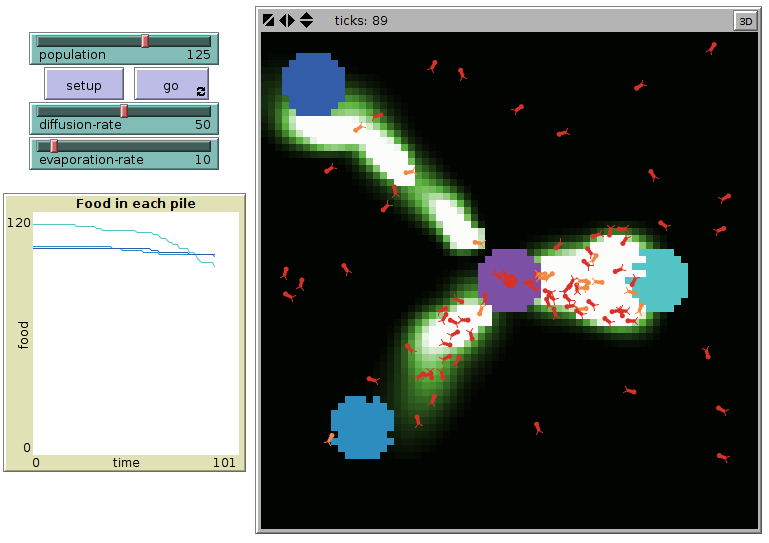
\includegraphics[scale=0.3]{Capture2.png}
\caption{Interface de la simulation}
\end{figure}
\end{frame}

\begin{frame}
\frametitle{Premières observations}
\begin{itemize}
\item Tendance à vider un tas de nourriture après l'autre avec les paramètres par défaut.
\item La diffusion et l'évaporation des phéromones sont nécessaires pour une récolte efficace.
\item Lorsque les phéromones ne persistent pas, tous les tas sont exploités en même temps et peu efficacement.
\end{itemize}
\end{frame}
\end{document}
